% --- PREAMBOLO LATEX ---
\documentclass[11pt,a4paper]{article}

\usepackage[utf8]{inputenc}
\usepackage[italian]{babel}

% Pacchetti per la matematica e la fisica
\usepackage{amsmath, amssymb, amsfonts}
\usepackage{cancel} % Utile per sbarrare i termini che si annullano

% Pacchetti per la grafica e l'impaginazione
\usepackage{graphicx}
\usepackage{geometry}
\usepackage{booktabs}
\usepackage{multirow}
\usepackage{sectsty}
\usepackage{float}
\usepackage{xcolor}

% Pacchetti per la lingua e la codifica
\usepackage[utf8]{inputenc}
\usepackage[italian]{babel}

% Pacchetti matematici indispensabili per Automatica
\usepackage{amsmath}
\usepackage{amssymb}
\usepackage{amsfonts}
\usepackage{mathtools}

% Pacchetti per immagini e formattazione
\usepackage{graphicx}
\usepackage{geometry}
\geometry{a4paper, top=2.5cm, bottom=2.5cm, left=2.5cm, right=2.5cm}
\usepackage{hyperref}
\usepackage{xcolor}
\usepackage{sectsty}
\allsectionsfont{\underline}
\setcounter{secnumdepth}{0}

\title{Appunti di Fondamenti di Automatica}
\author{Traduzione da slide del corso}
\date{}

\begin{document}

\maketitle
\tableofcontents
\newpage

\section{Introduzione}

\subsection{Sistema Fisico e suo Modello Matematico}
Ogni blocco di uno schema a blocchi rappresenta un sistema fisicamente esistente (per es. il processo in un sistema di controllo: gli studenti in aula, il corpo umano, la sala cinematografica, il lago), ma anche il suo modello matematico.

\begin{figure}[H]
    \centering
    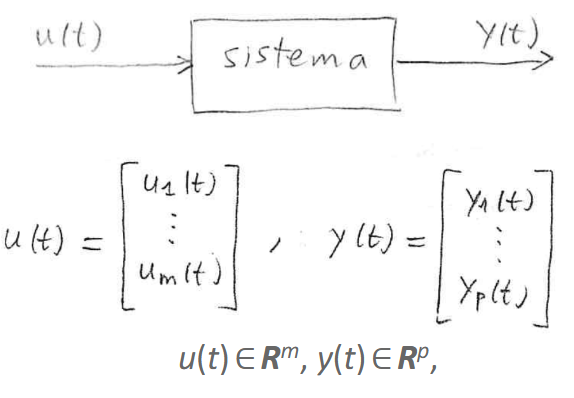
\includegraphics[width=0.3\linewidth]{immagini/2026-03-08-16-28-33.png}
    \end{figure}

Consideriamo:
\begin{itemize}
    \item $m$ variabili d'ingresso: $u_{1}(t), u_{2}(t), \dots, u_{m}(t)$
    \begin{itemize}
        \item (per es. se $m=2$, la variabile di controllo e un disturbo: voce del docente e rumore esterno all'aula; il comando dei muscoli e la forza peso; la portata d'aria condizionata e la temperatura esterna; l'apertura della diga e le precipitazioni)
    \end{itemize}
    \item $p$ variabili d'uscita: $y_{1}(t), y_{2}(t), \dots, y_{p}(t)$
    \begin{itemize}
        \item (per es. se $p=2$, la variabile controllata e un'altra variabile caratteristica: attenzione degli studenti e loro fame; posizione e velocità di un arto; temperatura e umidità della sala; livello e concentrazione di un inquinante)
    \end{itemize}
\end{itemize}

Le variabili esterne sono espresse in forma vettoriale come:
$$u(t)=\begin{bmatrix}u_{1}(t)\\ \vdots\\ u_{m}(t)\end{bmatrix} \in \mathbb{R}^{m}$$
$$y(t)=\begin{bmatrix}y_{1}(t)\\ \vdots\\ y_{p}(t)\end{bmatrix} \in \mathbb{R}^{p}$$

Questi segnali variano nel tempo $t$, che può essere:
\begin{itemize}
    \item \textbf{Continuo (t.c.)}: $t \in \mathbb{R}$
    \item \textbf{Discreto (t.d.)}: $t \in \mathbb{Z}$
\end{itemize}
La scelta tra tempo continuo e discreto è dettata dalla natura del segnale o da scelte modellistiche. $u(t)$ e $y(t)$ sono dette variabili esterne. Il sistema può avere altri ingressi (il cui effetto è trascurato) e altre variabili caratteristiche non misurate.

\subsection{Costruzione del Modello Matematico}
A partire dalle variabili esterne e sfruttando la conoscenza del sistema fisico, vogliamo formulare un legame matematico tra ingresso $u(t)$ e uscita $y(t)$. 
\textbf{Nota}: un modello (matematico) è per definizione una descrizione parziale e mai esatta della realtà. Un modello descrive gli aspetti del sistema fisico rilevanti agli scopi per cui il modello è sviluppato, trascurando altri aspetti.

Vi sono due classi fondamentali di modelli:
\begin{enumerate}
    \item Modello (sistema) non dinamico (algebrico)
    \item Modello (sistema) dinamico
\end{enumerate}

\subsubsection{Modello (Sistema) Non Dinamico (Algebrico)}
Definisce un legame istantaneo (valido in ogni $t$) tra l'ingresso $u(t)$, ed eventualmente l'istante di tempo $t$, e l'uscita $y(t)$:
$$y(t)=g(u(t),t)$$
dove $g$ è un vettore di $p$ funzioni (una funzione a valore vettoriale):
$$g(u,t)=\begin{bmatrix}g_{1}(u,t)\\ \vdots\\ g_{p}(u,t)\end{bmatrix}$$
Ciascuna funzione dipende da due argomenti $(u, t)$. Il primo è il vettore $u \in \mathbb{R}^{m}$ dei valori correnti degli ingressi; il secondo, opzionale, è l'istante $t$.

\subsubsection{Esempio di Modello Non Dinamico: la Legge di Ohm ($m=p=1$)}
\begin{figure}[H]
    \centering
    \begin{minipage}{0.3\textwidth}
        \centering
        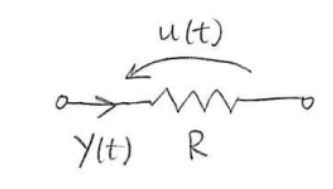
\includegraphics[width=\linewidth]{immagini/2026-03-08-16-33-27.png}
    \end{minipage}\hfill
    \begin{minipage}{0.65\textwidth}
        
        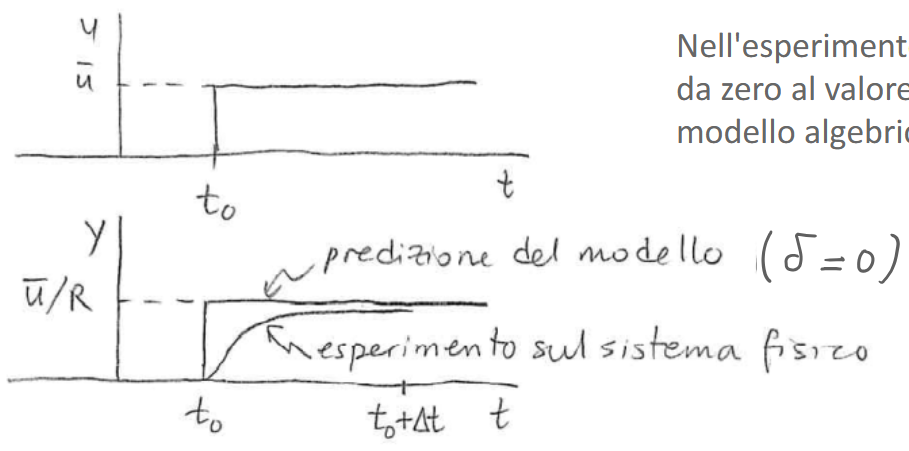
\includegraphics[width=\linewidth]{immagini/2026-03-08-16-33-09.png}
    \end{minipage}
\end{figure}

Nel caso base, $g$ non dipende esplicitamente da $t$:
$$y(t)=\frac{u(t)}{R}, \quad g(u,t)=\frac{u}{R}$$

Se la resistenza $R$ cambia nel tempo (ad esempio, perché sensibile all'escursione giornaliera di temperatura), allora $g$ dipende da $t$:
$$y(t)=\frac{u(t)}{R_{0}+\delta \sin(\omega t+\varphi)}, \quad g(u,t)=\frac{u}{R_{0}+\delta \sin(\omega t+\varphi)}, \quad R_{0}, \delta, \omega > 0$$

\textbf{Nota: il modello non è la realtà...}
Nell'esperimento fisico reale, se si applica un gradino di tensione al tempo $t_0$, la corrente non passa istantaneamente da zero al valore $\overline{u}/R$. C'è un transitorio $\Delta t$, quindi a rigore non si potrebbe scrivere un modello puramente algebrico. Tuttavia, se $\Delta t$ è sufficientemente piccolo da poter essere trascurato in molte applicazioni, la legge di Ohm risulta essere un buon modello ed è infatti molto usato.

\subsubsection{Modello (Sistema) Dinamico}
L'uscita $y(t)$ dipende anche dal valore di alcune \textbf{variabili interne} che descrivono lo stato del sistema all'istante $t$, dette \textbf{variabili di stato}.

$$y(t) = g(x(t), u(t), t) \quad \text{con } x(t) \in \mathbb{R}^{n}$$
Questa relazione è detta \textbf{trasformazione d'uscita}.

In forma vettoriale espansa si ha:
$$g(x, u, t) = \begin{bmatrix}g_{1}(x,u,t)\\ \vdots\\ g_{p}(x,u,t)\end{bmatrix}, \quad x(t) = \begin{bmatrix}x_{1}(t)\\ \vdots\\ x_{n}(t)\end{bmatrix}$$

Il numero $n \ge 1$ è detto \textbf{ordine} o \textbf{dimensione} del sistema.
L'idea è che lo stato $x$ all'istante $t$ riassuma l'effetto sull'uscita dei valori passati dell'ingresso (e dello stato stesso). Lo stato definisce quindi il legame dinamico tra ingresso e uscita.

\paragraph{Esempio di Modello Dinamico a tempo continuo (t.c.): un serbatoio ($m=p=1$)}

\begin{figure}[H]
    \centering
    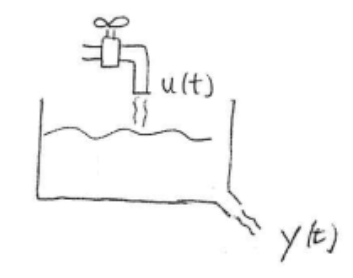
\includegraphics[width=0.2\linewidth]{immagini/2026-03-08-16-36-48.png}
    \end{figure}

\begin{itemize}
    \item $u(t)$ = portata entrante [kg/s]
    \item $y(t)$ = portata uscente [kg/s]
\end{itemize}

\textbf{Domanda 1:} se conosco $u(t)$ (oltre che l'istante $t$ e la fisica del sistema), posso determinare $y(t)$? \textbf{NO.}

\textbf{Domanda 2:} quali variabili di stato mi serve conoscere per determinare $y(t)$?
Scegliamo:
$$x(t) = \text{massa d'acqua contenuta [kg]}$$
$$y(t) = k \, x(t) \implies g(x, u, t) = k \, x$$
La portata uscente $y(t)$ è proporzionale alla pressione sul fondo, che è proporzionale al livello, e quindi alla massa se l'area della sezione è costante; $k$ è un parametro costante (coefficiente di deflusso del serbatoio). Si noti che la funzione $g$ non dipende dal tempo $t$ e nemmeno dall'ingresso $u$.

\textbf{Domanda 3:} la scelta fatta per $x(t)$ è sufficiente per definire lo stato del sistema?
Sì, se riesco a definire una regola di aggiornamento dello stato. Prima di vedere come, analizziamo un altro esempio.

\paragraph{Esempio di Modello Dinamico a tempo discreto (t.d.): un conto corrente ($m=p=1$)}

\begin{itemize}
    \item $u(t)$: deposito netto giornaliero (deposito - prelievo)
    \item $y(t)$: ammontare al mattino (prima di prelievo/deposito)
\end{itemize}

Ponendo:
$$x(t) = y(t) \implies g(x, u, t) = x$$
Questa è una scelta banale; la funzione $g$ non dipende esplicitamente da $t$ e nemmeno da $u$.

\subsection{Equazione di (Aggiornamento dello) Stato}
Lo stato $x(t)$, all'istante $t$, riassume l'effetto sull'uscita $y(t)$ dei valori passati di ingresso e stato stesso.

Noto lo stato $x(t_0)$ ad un \textbf{istante iniziale} $t_0$ e noto il segnale d'ingresso nell'intervallo $[t_0, t)$ che va fino ad un \textbf{istante finale} $t > t_0$ (escluso), deve essere possibile determinare lo stato $x(t')$ in tutto l'intervallo $[t_0, t]$ ($t' \in [t_0, t]$), in particolare lo stato finale $x(t)$. In questo modo anche l'uscita $y(t')$ è nota in tutto l'intervallo.

Come si fa? Formulando l'\textbf{equazione di stato}:

\begin{itemize}
    \item \textbf{t.c.: equazioni differenziali}
    $$\frac{d}{dt}x(t) = \dot{x}(t) = f(x(t), u(t), t)$$
    
    \item \textbf{t.d.: equazioni alle differenze}
    $$x(t+1) = f(x(t), u(t), t)$$
\end{itemize}

In forma vettoriale:
$$f(x, u, t) = \begin{bmatrix} f_1(x,u,t) \\ \vdots \\ f_n(x,u,t) \end{bmatrix}$$

\textbf{Domanda 3:} la scelta di $x(t)$ è una buona definizione di stato?
Sì se riesco a definire $f$, altrimenti devo aggiungere delle variabili di stato.

\textbf{Esempi ripresi:}
\begin{itemize}
    \item \textbf{Serbatoio ($n=1$):}
    $$\dot{x} = u - kx \implies f(x, u, t) = u - kx$$
    Basato sulla conservazione della massa: $(x(t+dt) = x(t) + u(t)dt - kx(t)dt)$.
    
    \item \textbf{Conto corrente ($n=1$):}
    $$x(t+1) = (x(t) + u(t))(1+\rho) \implies f(x, u, t) = (x+u)(1+\rho)$$
    Dove $0 < \rho < 1$ è il tasso giornaliero d'interesse.
\end{itemize}

\subsubsection{Esempio: Controllo di temperatura di una sala cinematografica}



\begin{figure}[H]
    \centering
    \begin{minipage}{0.3\textwidth}
        \centering
        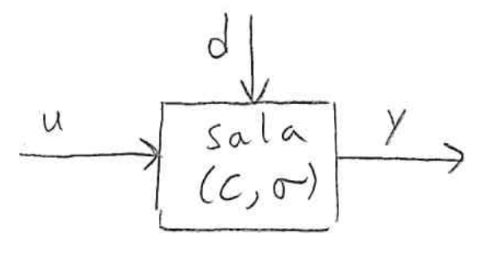
\includegraphics[width=\linewidth]{immagini/2026-03-08-16-44-27.png}
    \end{minipage}\hfill
    \begin{minipage}{0.65\textwidth}
        \textbf{Variabili:}
        \begin{itemize}
            \item $y(t)$: temperatura della sala
            \item $y^\circ$: temperatura desiderata (costante)
            \item $d$: temperatura esterna (costante)
            \item $u(t)$: flusso di calore di condizionamento
        \end{itemize}
        
        \textbf{Parametri:}
        \begin{itemize}
            \item $C$: capacità termica della sala
            \item $\sigma$: coefficiente di scambio termico
        \end{itemize}
    \end{minipage}
\end{figure}

Modello matematico del processo (un'equazione differenziale lineare):
$$C\frac{d}{dt}y(t) = \sigma(d(t) - y(t)) + u(t)$$
Ovvero: variazione di calore = bilancio dei flussi di calore.
In questo caso, $y(t) = x(t)$ è la variabile di stato ($n=1$).

\subsubsection{Esempio: La legge di Newton}
Questo è un caso in cui il procedimento visto risponde inizialmente \textbf{NO alla Domanda 3}. È un esempio storico (fine 1600), il primo sistema dinamico a t.c., in quanto Newton ha introdotto (con Leibniz) il calcolo infinitesimale.

\begin{figure}[H]
    \centering
    \begin{minipage}{0.3\textwidth}
        \centering
        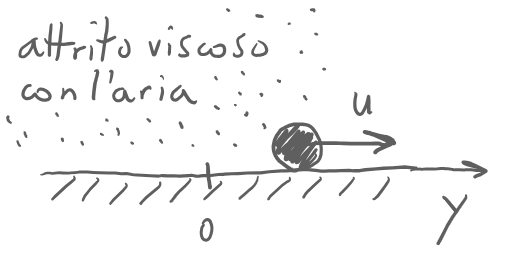
\includegraphics[width=\linewidth]{immagini/2026-03-08-16-47-56.png}
    \end{minipage}\hfill
    \begin{minipage}{0.65\textwidth}
        \begin{itemize}
            \item $u(t)$: forza motrice (positiva verso destra, frenante se discorde alla velocità)
            \item $y(t)$: posizione (sull'asse $y$ orientato verso destra)
            \item Parametri: $m$ massa della pallina; $h$ coefficiente di attrito viscoso.
        \end{itemize}
    \end{minipage}
\end{figure}

\textit{Nota:} Più precisamente la pallina è considerata un punto materiale. Consideriamo solo l'attrito viscoso dell'aria e non quello radente o volvente. Nel caso orizzontale la forza di gravità è compensata dalla reazione vincolare.

\textbf{Domanda 2:} quali variabili di stato serve conoscere per determinare $y(t)$?
È sufficiente la scelta banale: $x(t) = \text{posizione} \implies y(t) = x(t) \implies g(x, u, t) = x$.

\textbf{Domanda 3:} la scelta di $x(t)$ è una buona definizione di stato?
Proviamo a scrivere l'equazione di stato:
$$\frac{d}{dt}x(t) = \text{velocità} = f(x(t), u(t), t) \text{ ?}$$
\textbf{No}, non riesco a esprimere la velocità come una funzione di posizione e forza all'istante $t$!
Quindi la aggiungo come variabile di stato $x_2$ (la posizione diventa $x_1$).

Dalla Legge di Newton $F = m \cdot a$:
$$\dot{x}_1(t) = x_2(t) \implies f_1(x, u, t) = x_2$$
$$\dot{x}_2(t) = \text{accelerazione} = \frac{1}{m}(u(t) - h x_2(t)) \implies f_2(x, u, t) = \frac{1}{m}(u - h x_2)$$

\textit{Nota:} è noto che posizione e velocità dei corpi in movimento descrivono lo stato di un sistema meccanico.

\subsubsection{Esempio: L'allevamento di Fibonacci (XIII sec.)}
Il primo sistema dinamico a t.d. 

\textbf{Regole del sistema fisico:}
\begin{itemize}
    \item I conigli sono giovani nel primo mese di vita e adulti a partire dal secondo.
    \item Ogni coppia (maschio-femmina) adulta genera una nuova coppia ogni fine mese.
    \item I conigli non muoiono mai, ma Fibonacci ne preleva $u(t)$ coppie adulte alla fine del mese $t$ (dopo la riproduzione).
    \item A metà mese, osserva il totale di coppie $y(t)$.
\end{itemize}
\textit{Nota:} a t.d. è importante la temporizzazione degli eventi!

\textbf{Domanda 2:} quali variabili di stato mi serve conoscere per determinare $y(t)$?
Tentativo: $x(t) = \text{num. totale di coppie} \implies y(t) = x(t) \implies g(x, u, t) = x$.

\textbf{Domanda 3:} la scelta di $x(t)$ è una buona definizione di stato?
Equazione di stato:
$$x(t+1) = x(t) + \underbrace{\text{nuove coppie nate alla fine del mese } t}_{\text{pari alle coppie adulte del mese } t} - u(t)$$
Poiché non posso distinguere le coppie adulte dal solo totale $x(t)$, la scelta non va bene. 

\textbf{Formulazione 1:} Scegliamo $x_1(t)$ = num. totale coppie; $x_2(t)$ = coppie adulte nel mese $t$ (osservate a metà mese):
$$x_1(t+1) = x_1(t) + x_2(t) - u(t)$$
$$x_2(t+1) = x_2(t) - u(t) + \underbrace{x_1(t) - x_2(t)}_{\text{coppie giovani nel mese } t} = x_1(t) - u(t)$$
$$y(t) = x_1(t)$$

\textbf{Formulazione 2 (più tipica):} $x_1(t)$ = coppie giovani e $x_2(t)$ = coppie adulte nel mese $t$.
$$x_1(t+1) = x_2(t)$$
$$x_2(t+1) = x_1(t) + x_2(t) - u(t)$$
$$y(t) = x_1(t) + x_2(t)$$

\textit{Nota:} la scelta delle variabili di stato non è univoca! Nei modelli demografici con struttura d'età è tipico usare una var. di stato per ogni classe di età.

La sequenza di Fibonacci: $y(t)$ nel caso senza prelievo partendo da una coppia giovane:

\begin{table}[htbp]
    \centering
    \begin{tabular}{c|cccccccc}
        $t$ & 0 & 1 & 2 & 3 & 4 & 5 & 6 & 7 \\
        \hline
        $x_1(t)$ & 1 & 0 & 1 & 1 & 2 & 3 & 5 & 8 \\
        $x_2(t)$ & 0 & 1 & 1 & 2 & 3 & 5 & 8 & 13 \\
        \hline
        $y(t)$ & 1 & 1 & 2 & 3 & 5 & 8 & 13 & 21
    \end{tabular}
\end{table}

\subsection{Modello (Sistema) Dinamico: Riassumendo}
\begin{itemize}
    \item \textbf{t.c. (equazione di stato):} $\dot{x}(t) = f(x(t), u(t), t)$
    \item \textbf{t.d. (equazione di stato):} $x(t+1) = f(x(t), u(t), t)$
\end{itemize}
\textbf{Trasformazione d'uscita:}
$$y(t) = g(x(t), u(t), t)$$

\textit{Nota:} a t.c. "dimenticheremo" spesso di indicare la dipendenza dal tempo:
$$ \begin{cases} 
\dot{x} = f(x, u, t) \\ 
y = g(x, u, t) 
\end{cases} $$

\subsection{Classificazione dei Sistemi Dinamici}
\begin{itemize}
    \item \textbf{Deterministici:} nessun evento casuale; stato iniziale $x(t_0)$ e ingresso $u(\tau)$ (con $\tau \ge t_0$) determinano il futuro.
    \item \textbf{Stocastici:} le funzioni $f$ e $g$ dipendono anche da qualche processo casuale.
    \item \textbf{Dimensione finita ($n$ finito):} $x(t) \in \mathbb{R}^n$, l'equazione di stato è ordinaria (ODE).
    \item \textbf{Dimensione infinita ($n = \infty$):} un esempio classico è l'equazione del calore, in cui lo stato è la temperatura in ogni punto di un corpo.
\end{itemize}

\begin{figure}[H]
    \centering
    \begin{minipage}{0.3\textwidth}
        \centering
        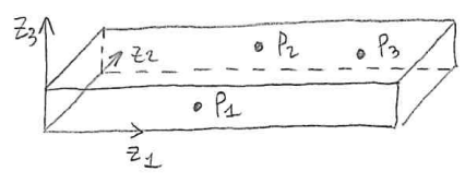
\includegraphics[width=\linewidth]{immagini/2026-03-08-16-58-12.png}
    \end{minipage}\hfill
    \begin{minipage}{0.65\textwidth}
        $$ x(t) = \begin{bmatrix} x_1(t) \\ x_2(t) \\ x_3(t) \\ \vdots \end{bmatrix} 
        \begin{matrix} 
        \text{temp. in } P_1 \\ 
        \text{temp. in } P_2 \\ 
        \text{temp. in } P_3 \\ 
        \vdots 
        \end{matrix} $$
    \end{minipage}
\end{figure}
Lo stato al tempo $t$ è una funzione delle 3 coordinate spaziali $(z_1, z_2, z_3)$. Si ha quindi che $x(t) \in$ spazio funzionale.
L'equazione di stato è tipicamente un'equazione differenziale (t.c.) o alle differenze (t.d.) alle derivate parziali (PDE).

\subsubsection{Esempio: Il ritardatore a t.c.}
È l'unico sistema dinamico a dimensione infinita che considereremo.

\begin{figure}[H]
    \centering
    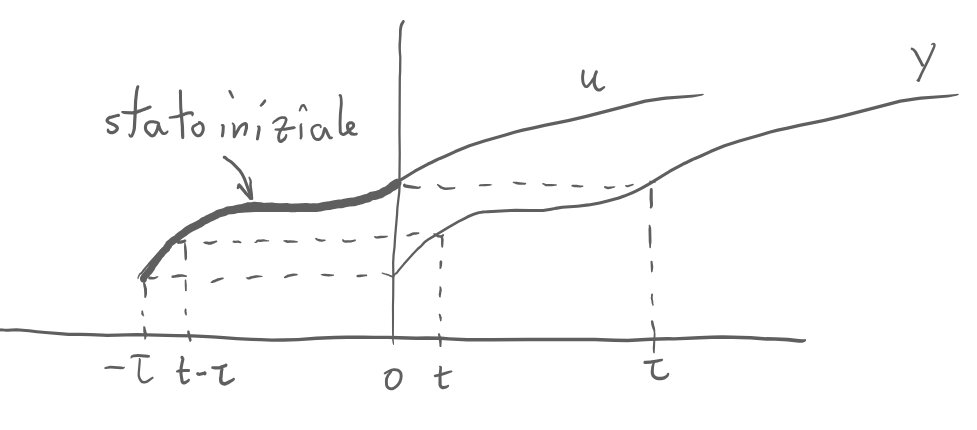
\includegraphics[width=0.6\linewidth]{immagini/2026-03-08-17-04-23.png}
    \end{figure}

$$y(t) = u(t - \tau)$$
Lo stato $x(t)$ è l'intera porzione di segnale $u(t')$ per $t' \in [t-\tau, t]$.

\subsubsection{Dimensione finita ($n$ finito)}
\begin{figure}[H]
    \centering
    \begin{minipage}{0.3\textwidth}
        \centering
        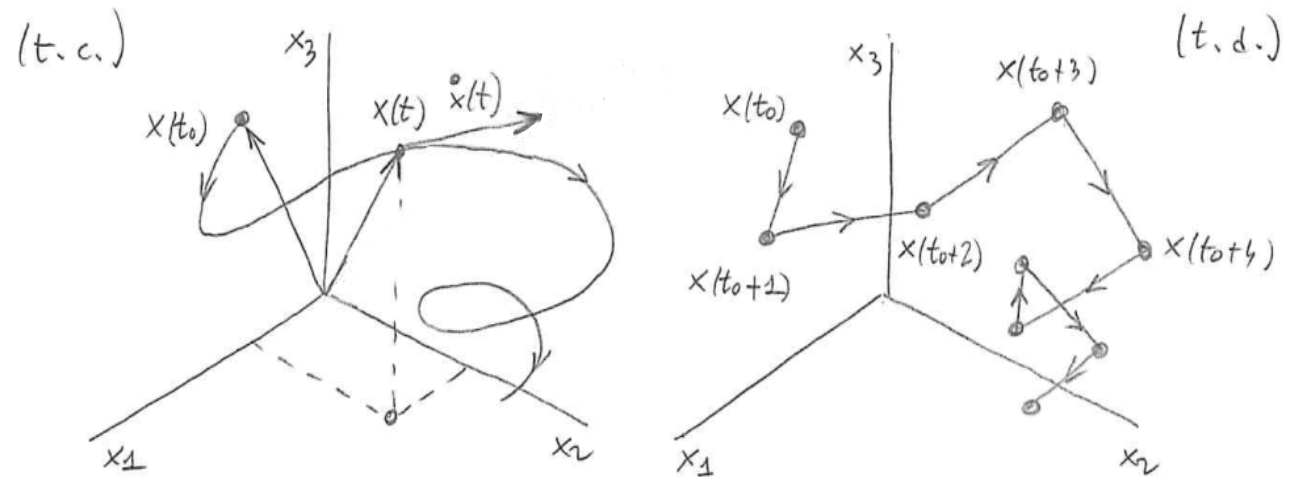
\includegraphics[width=\linewidth]{immagini/2026-03-08-17-11-24.png}
    \end{minipage}\hfill
    \begin{minipage}{0.65\textwidth}
        $x(t) \in \mathbb{R}^n$, dove $\mathbb{R}^n$ è lo \textbf{spazio di stato}.
        \textbf{Interpretazione geometrica:} lo stato è un punto che si muove nello spazio di stato. Parte dallo stato (o condizione) iniziale $x(t_0)$ e percorre una \textbf{traiettoria}.
        
        \textit{Nota:} a t.c. il vettore $\dot{x}(t)$ (disegnato a partire dalla punta del vettore $x(t)$) è tangente alla traiettoria nel verso di avanzamento del tempo e rappresenta il vettore "velocità" con cui si muove il punto di stato. \\
        \textit{Nota:} a t.d. i segmenti che uniscono i punti successivi della traiettoria hanno solo utilità grafica.
    \end{minipage}
\end{figure}

\subsection{Il quadro delle traiettorie}
Un insieme di traiettorie dalle quali sia possibile capire, qualitativamente, tutte le altre.

\subsubsection{Esempio: Newton senza attrito ($h=0$)}

\begin{figure}[H]
    \centering
    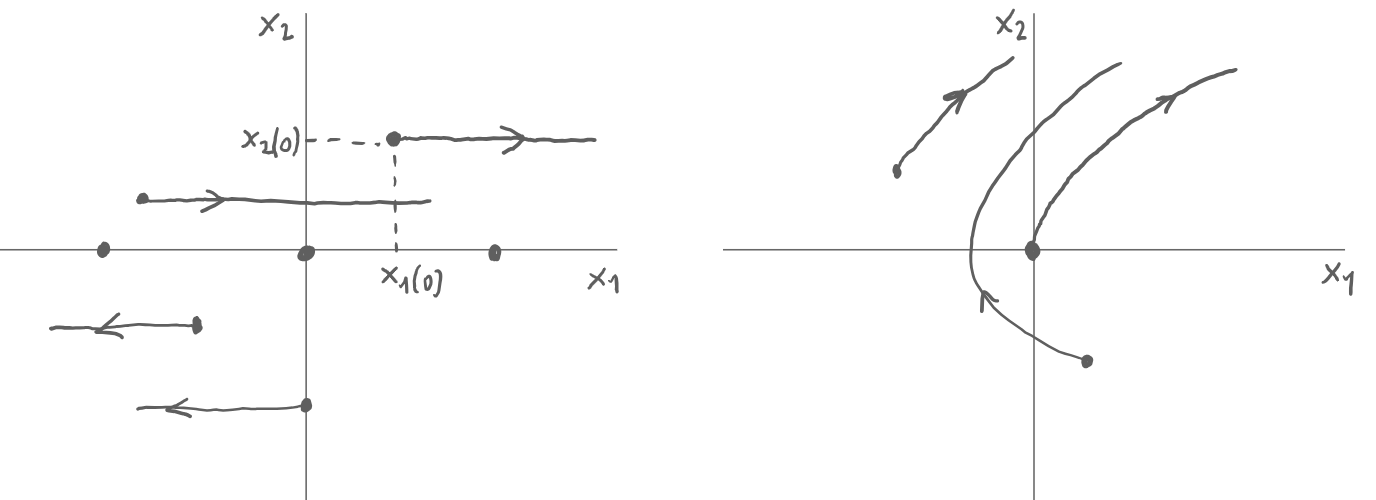
\includegraphics[width=0.7\linewidth]{immagini/2026-03-08-17-11-58.png}
    \end{figure}

\begin{itemize}
    \item \textbf{Senza forza motrice ($u(t)=0$):} Moto rettilineo uniforme.
    $$ \begin{bmatrix} \dot{x}_1 \\ \dot{x}_2 \end{bmatrix} = \begin{bmatrix} x_2 \\ 0 \end{bmatrix} $$
    \item \textbf{Con forza motrice costante ($u(t)=\bar{u}>0$):} Moto uniformemente accelerato.
    $$ \begin{bmatrix} \dot{x}_1 \\ \dot{x}_2 \end{bmatrix} = \begin{bmatrix} x_2 \\ \frac{\bar{u}}{m} \end{bmatrix} $$
\end{itemize}

\subsubsection{Esempio: Newton con attrito ($h>0$)}

\begin{figure}[H]
    \centering
    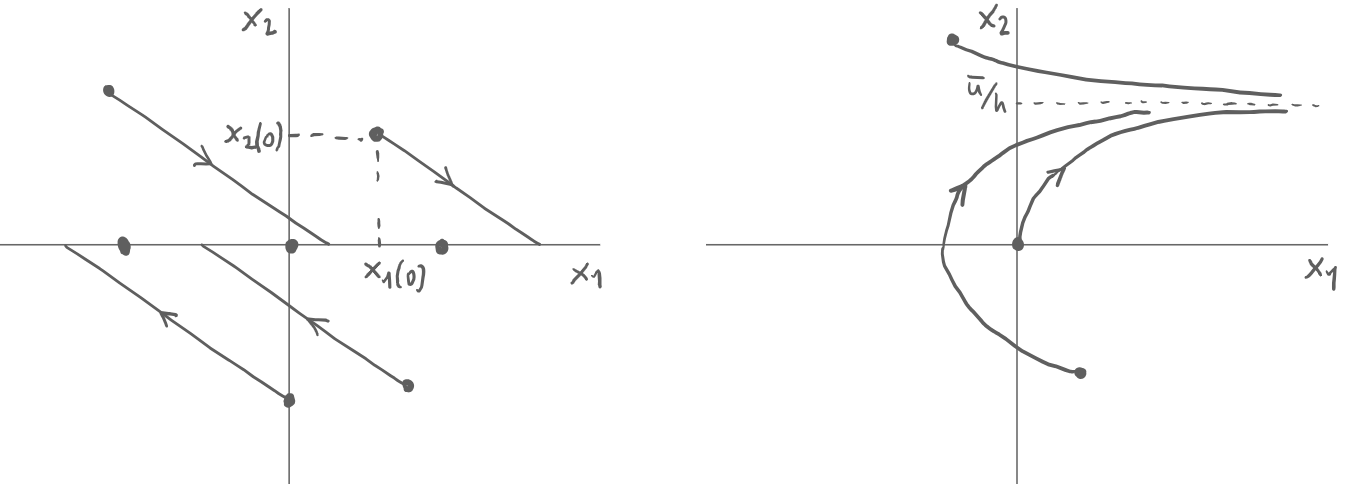
\includegraphics[width=0.7\linewidth]{immagini/2026-03-08-17-13-06.png}
    \end{figure}

\begin{itemize}
    \item \textbf{Senza forza motrice ($u(t)=0$):} Arresto (traiettorie rettilinee!).
    $$ \begin{bmatrix} \dot{x}_1 \\ \dot{x}_2 \end{bmatrix} = \begin{bmatrix} x_2 \\ -\frac{h}{m}x_2 \end{bmatrix} $$
    \item \textbf{Con forza motrice costante ($u(t)=\bar{u}>0$):} Caduta con velocità limite (pari a $\bar{u}/h$).
    $$ \begin{bmatrix} \dot{x}_1 \\ \dot{x}_2 \end{bmatrix} = \begin{bmatrix} x_2 \\ \frac{1}{m}(\bar{u} - hx_2) \end{bmatrix} $$
\end{itemize}

\subsubsection{Sistemi Propri e Impropri}

\begin{figure}[H]
    \centering
    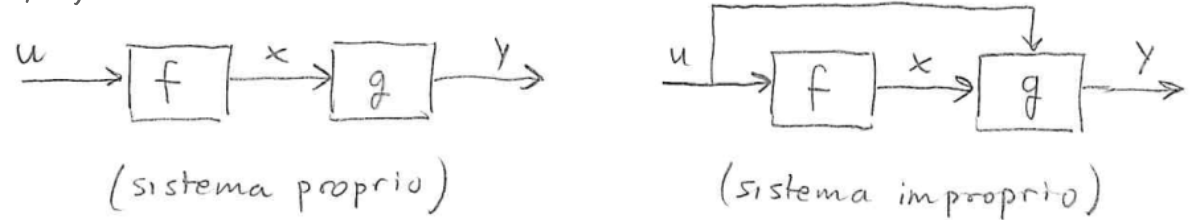
\includegraphics[width=0.8\linewidth]{immagini/2026-03-08-17-45-27.png}
    \end{figure}

\begin{itemize}
    \item \textbf{Sistemi propri [impropri]:} è assente [presente] un legame istantaneo tra ingresso e uscita.
    \item $g(x, u, t)$ non dipende [dipende] dall'argomento $u$.
\end{itemize}

\textit{Nota:} alcuni testi usano "strettamente proprio" e "non strettamente proprio", riservando il termine "improprio" ad una formulazione approssimata nel dominio della frequenza.

\subsubsection{Altre Classificazioni}
\begin{itemize}
    \item \textbf{Sistemi (tempo) invarianti [varianti]:} la dinamica non dipende [dipende] dall'istante iniziale $t_0$.
    $f(x, u, t)$ e $g(x, u, t)$ non dipendono [almeno una dipende] dall'argomento $t$. \\
    \textit{Nota:} nei sistemi tempo invarianti, l'istante iniziale è per convenzione fissato in $t_0 = 0$.
    
    \item \textbf{Sistemi autonomi:} non hanno ingressi ($m = 0$) o, equivalentemente, gli ingressi sono costanti (e considerati come parametri; per es. Newton con forza motrice costante).
    $f(x, u, t)$ e $g(x, u, t)$ non dipendono dall'argomento $u$.
    
    \item \textbf{Sistemi SISO (Single-Input-Single-Output):} $m = 1, p = 1$.
    \item \textbf{Sistemi MIMO (Multiple-Input-Multiple-Output):} $m \ge 2$ e/o $p \ge 2$.
\end{itemize}

\subsection{Sistemi Lineari}
Nei sistemi lineari, le funzioni $f(x, u, t)$ e $g(x, u, t)$ sono combinazioni lineari di $x$ e $u$:
$$ f(x, u, t) = A(t)x + B(t)u $$
$$ g(x, u, t) = C(t)x + D(t)u $$

Dove le matrici di funzioni del tempo hanno le seguenti dimensioni:
\begin{itemize}
    \item $A(t) = [a_{ij}(t)]$ matrice $n \times n$
    \item $B(t) = [b_{ij}(t)]$ matrice $n \times m$
    \item $C(t) = [c_{ij}(t)]$ matrice $p \times n$
    \item $D(t) = [d_{ij}(t)]$ matrice $p \times m$
\end{itemize}

\textit{Nota 1:} gli elementi delle matrici possono dipendere dal tempo. Se almeno un elemento è funzione di $t$, il sistema è tempo-variante, altrimenti è invariante. \\
\textit{Nota 2:} la linearità è richiesta rispetto a $x$ e $u$ congiuntamente, quindi, per es., i prodotti $x_i u_j$ sono delle non-linearità (mentre non lo sono i prodotti $x_i t$).

\subsubsection{Esempio di Sistema Non Lineare: La crescita logistica}
Modello classico in ecologia e economia.
\begin{itemize}
    \item \textbf{t.c.:} $\dot{x} = rx(1 - x/K)$
    A bassa densità ($x \ll K$), la biomassa cresce proporzionalmente a quanta ce n'è. Ad alta densità, la competizione per risorse (termine non lineare $-rx^2/K$) domina e rende negativa la derivata $\dot{x}$ ($x$ diminuisce).
    \item \textbf{t.d.:} $x(t+1) = x(t) + rx(t)(1 - x(t)/K)$ dove $x(t)$ è il capitale di un'azienda nel periodo $t$.
\end{itemize}

\subsubsection{Esempi di Sistemi Lineari}
\textbf{Newton è lineare, proprio, invariante, SISO}
$$ \begin{cases} \dot{x}_1 = x_2 \\ \dot{x}_2 = \frac{1}{m}(u - hx_2) \end{cases} \implies \begin{bmatrix} \dot{x}_1 \\ \dot{x}_2 \end{bmatrix} = \underbrace{\begin{bmatrix} 0 & 1 \\ 0 & -\frac{h}{m} \end{bmatrix}}_{A(2\times2)} \begin{bmatrix} x_1 \\ x_2 \end{bmatrix} + \underbrace{\begin{bmatrix} 0 \\ \frac{1}{m} \end{bmatrix}}_{b(2\times1)} u $$
$$ y = x_1 \implies y = \underbrace{\begin{bmatrix} 1 & 0 \end{bmatrix}}_{c^T(1\times2)} \begin{bmatrix} x_1 \\ x_2 \end{bmatrix} + \underbrace{[0]}_{d(1\times1)} u $$
\textit{Notazione:} lettere maiuscole = matrici; lettere minuscole = scalari ($1\times1$) e vettori colonna.

\textbf{Anche Fibonacci è lineare, proprio, invariante, SISO}
$$ \begin{cases} x_1(t+1) = x_2(t) \\ x_2(t+1) = x_1(t) + x_2(t) - u(t) \end{cases} \implies \begin{bmatrix} x_1(t+1) \\ x_2(t+1) \end{bmatrix} = \underbrace{\begin{bmatrix} 0 & 1 \\ 1 & 1 \end{bmatrix}}_{A} \begin{bmatrix} x_1(t) \\ x_2(t) \end{bmatrix} + \underbrace{\begin{bmatrix} 0 \\ -1 \end{bmatrix}}_{b} u(t) $$
$$ y(t) = x_1(t) + x_2(t) \implies y(t) = \underbrace{\begin{bmatrix} 1 & 1 \end{bmatrix}}_{c^T} \begin{bmatrix} x_1(t) \\ x_2(t) \end{bmatrix} + \underbrace{[0]}_{d} u(t) $$
\textit{Nota:} anche il serbatoio e il conto corrente sono sistemi lineari (del primo ordine, $n=1$, $A$ è scalare); anche il ritardatore lo è (lo capiremo più avanti, vedi sovrapposizione cause ed effetti).

\subsection{Nota sulla definizione di stato e temporizzazione a t.d.}
Noto lo stato $x(t_0)$ ad un istante iniziale $t_0$ e noto il segnale d'ingresso nell'intervallo $[t_0, t)$ che va fino ad un istante finale $t > t_0$ (escluso), deve essere possibile determinare lo stato $x(t')$ in tutto l'intervallo $[t_0, t]$.
Per scelta modellistica, lo stato riassume l'effetto sull'uscita dei valori passati dell'ingresso. Il legame istantaneo tra ingresso e uscita, se presente, è descritto nella trasformazione d'uscita.
\textbf{Non è quindi accettabile una definizione di stato che sia influenzata istantaneamente dall'ingresso.}

\textbf{Esempio: il conto corrente}
\begin{itemize}
    \item $u(t)$: deposito netto giornaliero
    \item $y(t)$: saldo a fine giornata (prima dell'applicazione dell'interesse)
\end{itemize}
Se usassimo la scelta apparentemente comoda e banale $x(t) = y(t)$, avremmo:
$$ x(t+1) = (1+\rho)x(t) + \underbrace{u(t+1)}_{\text{errato}} $$
Questo vìola il principio appena esposto. La scelta corretta è quindi:
$$ x(t) = \text{saldo a inizio giornata} $$
che rende il sistema ben formulato (e improprio):
$$ y(t) = x(t) + u(t) $$
$$ x(t+1) = (1+\rho)(x(t) + u(t)) $$

\subsection{Riassumendo}
I sistemi (dinamici, deterministici, dimensione finita) lineari, invarianti, SISO sono descritti dalle seguenti equazioni:
\begin{itemize}
    \item \textbf{Tempo Continuo (t.c.):}
    $$ \dot{x} = Ax + bu $$
    $$ y = c^T x + du $$
    \item \textbf{Tempo Discreto (t.d.):}
    $$ x(t+1) = Ax(t) + bu(t) $$
    $$ y(t) = c^T x(t) + du(t) $$
\end{itemize}

\section{Formulazione del modello}

\subsection{Dal Modello Interno al Modello Esterno (ARMA)}

\textbf{MODELLO INTERNO:} prima formulazione, qui considerata per sistema SISO ($m = 1, p = 1$)
\begin{itemize}
    \item \textbf{t.c.:} $\dot{x} = Ax + bu$
    \item \textbf{t.d.:} $x(t+1) = Ax(t) + bu(t)$
\end{itemize}
$$ y(t) = c^T x(t) + du(t) $$

\textbf{MODELLO ESTERNO (ARMA):} seconda formulazione, sempre SISO (oppure uno per ogni coppia $(y_i, u_j)$)
\begin{itemize}
    \item \textbf{t.d.:}
    $$ y(t) + \alpha_1 y(t-1) + \alpha_2 y(t-2) + \dots + \alpha_n y(t-n) = \beta_0 u(t) + \beta_1 u(t-1) + \beta_2 u(t-2) + \dots + \beta_n u(t-n) $$
\end{itemize}

Possiamo scriverlo in forma compatta evidenziando le due parti:
$$ y(t) = \underbrace{-\sum_{i=1}^n \alpha_i y(t-i)}_{\text{AR (auto-regressive)}} + \underbrace{\sum_{i=0}^n \beta_i u(t-i)}_{\text{MA (moving average)}} $$

$n$ è l'ordine del modello ARMA (con $\alpha_n$ e $\beta_n$ non entrambi nulli) ed è $\le$ dell'ordine del modello interno.

A volte è più utile scrivere il modello "in avanti nel tempo", tanto l'equazione vale per ogni istante $t$:
$$ y(t+n) + \alpha_1 y(t+n-1) + \alpha_2 y(t+n-2) + \dots + \alpha_n y(t) = \beta_0 u(t+n) + \beta_1 u(t+n-1) + \beta_2 u(t+n-2) + \dots + \beta_n u(t) $$

\begin{itemize}
    \item \textbf{t.c.:}
    $$ y^{(n)}(t) + \alpha_1 y^{(n-1)}(t) + \alpha_2 y^{(n-2)}(t) + \dots + \alpha_n y^{(0)}(t) = \beta_0 u^{(n)}(t) + \beta_1 u^{(n-1)}(t) + \beta_2 u^{(n-2)}(t) + \dots + \beta_n u^{(0)}(t) $$
\end{itemize}
Dove: $y^{(k)}(t) = \frac{d^k}{dt^k}y(t)$.

\subsubsection{Esempi di formulazione ARMA}

\textbf{NEWTON ($y$: posizione, $u$: forza motrice)}
$$ y^{(1)} = \text{velocità} = \text{non riesco a ottenerla come combinazione di } y^{(0)}, u^{(0)} \text{ e } u^{(1)} $$
$$ y^{(2)} = \text{accelerazione} = \text{da scrivere come comb. di } y^{(0,1)}, u^{(0,1,2)} = \frac{1}{m}(-h y^{(1)} + u) $$
Riordinando i termini si ottiene:
$$ \alpha_1 = \frac{h}{m}, \quad \alpha_2 = 0, \quad \beta_0 = 0, \quad \beta_1 = 0, \quad \beta_2 = \frac{1}{m} $$

\noindent
\textbf{FIBONACCI ($y(t)$: totale coppie, $u(t)$: prelievo coppie adulte)}
$$ y(t) = y(t-1) + \underbrace{(\text{coppie nate alla fine del mese } t-1)}_{= \text{coppie adulte nel mese } t-1} - u(t-1) $$
Poiché le coppie adulte nel mese $t-1$ equivalgono al totale delle coppie nel mese $t-2$ meno il prelievo a fine mese, il termine diventa: $y(t-2) - u(t-2)$.
Quindi:
$$ y(t) = y(t-1) + y(t-2) - u(t-2) - u(t-1) $$
In avanti nel tempo (anticipando di 2 passi):
$$ y(t+2) - y(t+1) - y(t) = -u(t+1) - u(t) $$
Da cui si ricava:
$$ \alpha_1 = -1, \quad \alpha_2 = -1, \quad \beta_0 = 0, \quad \beta_1 = -1, \quad \beta_2 = -1 $$

\textit{Nota:} solitamente, ci viene più naturale ragionare sulla formulazione interna.

\subsection{Notazione Polinomiale}

Introduciamo il simbolo $p$:
\begin{itemize}
    \item $s$ \textbf{(t.c.):} rappresenta la derivata rispetto al tempo, $s y(t) = \frac{d}{dt}y(t) = y^{(1)}(t)$, e $s^k y(t) = \frac{d^k}{dt^k}y(t) = y^{(k)}(t)$.
    \item $z$ \textbf{(t.d.):} rappresenta l'anticipo di un passo, $z y(t) = y(t+1)$, e $z^k y(t) = y(t+k)$.
\end{itemize}

Sostituendo l'operatore $p$ nelle equazioni (sia t.c. che t.d.):
$$ p^n y(t) + \alpha_1 p^{n-1} y(t) + \dots + \alpha_n y(t) = \beta_0 p^n u(t) + \beta_1 p^{n-1} u(t) + \dots + \beta_n u(t) $$

Raccogliendo $y(t)$ e $u(t)$:
$$ \underbrace{(p^n + \alpha_1 p^{n-1} + \dots + \alpha_n)}_{D(p)} y(t) = \underbrace{(\beta_0 p^n + \beta_1 p^{n-1} + \dots + \beta_n)}_{N(p)} u(t) $$

Otteniamo quindi la notazione sintetica:
$$ D(p) y(t) = N(p) u(t) \quad \text{ovvero} \quad Dy = Nu $$

\textbf{NOTA:} $D(p)$ è un polinomio di grado $n$ \textbf{monico} (coefficiente del monomio di grado massimo $= 1$). $N(p)$ è un polinomio di grado $\le n$.

\subsection{Funzione di Trasferimento}

\textbf{FUNZIONE DI TRASFERIMENTO} (F.d.T., terza formulazione, SISO): 
$$ G(p) = \frac{N(p)}{D(p)} $$
Notazione sintetica: $y = G u$.

\textbf{NOTA:} cosa significa avere il simbolo $p$ a denominatore?
Intuitivamente:
\begin{itemize}
    \item t.c.: $s^{-1} u(t) = \int_0^t u(\tau) d\tau$
    \item t.d.: $z^{-1} u(t) = u(t-1)$
\end{itemize}

Ma cosa significa dividere $u$ per un polinomio in $p$?
Il significato corretto è in "frequenza": la F.d.T. è il fattore che lega le trasformate di Laplace (t.c.) e Z (t.d.) di $u$ e $y$, dove $p$ è la variabile complessa della trasformata:
$$ Y(p) = G(p) U(p) $$
Nel dominio della frequenza, il legame tra $u$ e $y$ è \textbf{algebrico}!

Le trasformate descrivono il contributo al segnale di segnali base di tipo armonico ($\sin$ per la trasformata di Fourier; $\exp \cdot \sin$ per Laplace e Z). La variabile complessa $p$ descrive il segnale base (esponenziale e frequenza della parte sinusoidale); il numero complesso $U(p)$ definisce il suo contributo in $u$ (modulo = ampiezza; angolo = fase sin) e $G(p)$ ci dice come questo contributo viene trasformato dal sistema nel corrispondente contributo a $y$.

\begin{figure}[H]
    \centering
    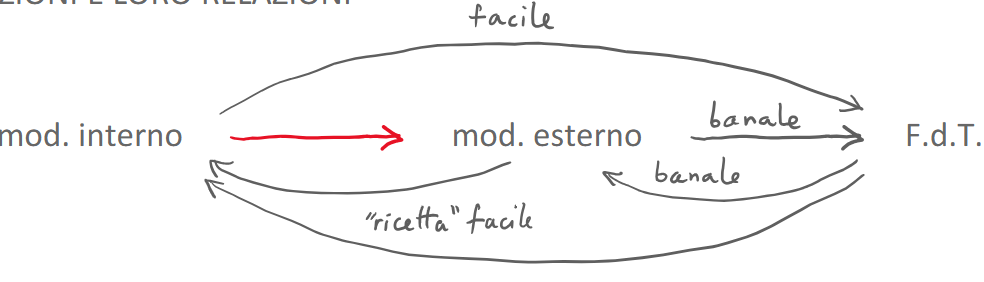
\includegraphics[width=0.7\linewidth]{immagini/2026-03-08-18-12-09.png}
    \end{figure}

\subsection{Da Modello Interno a Esterno: i due classici esempi}

\textbf{Procedura:} sfruttando l'operatore $p$ (ovvero $s$ per t.c. e $z$ per t.d.), l'equazione di stato diventa \textit{algebrica}! Vanno eliminate le variabili di stato dalla trasformazione d'uscita, risolvendo le $n$ equazioni di stato nelle $n$ incognite $x_i$ in funzione di $u$.

\subsubsection{Newton}
\begin{itemize}
    \item Modello ARMA: $y^{(2)} + \frac{h}{m}y^{(1)} = \frac{1}{m}u$
    \item Polinomi: $D(s) = s^2 + \frac{h}{m}s, \quad N(s) = \frac{1}{m}$
    \item F.d.T.: $G(s) = \frac{1}{ms(s + h/m)}$
\end{itemize}

\textit{Svolgimento con operatore $s$:}
$$ \begin{cases}
s x_1 = x_2 \\
s x_2 = -\frac{h}{m}x_2 + \frac{1}{m}u \implies \left(s + \frac{h}{m}\right)x_2 = \frac{u}{m}
\end{cases} $$
Sostituendo nella trasformazione d'uscita $y = x_1$:
\begin{align*}
\text{Moltiplico per } s&: s y = s x_1 = x_2 \\
\text{Moltiplico per } \left(s + \frac{h}{m}\right)&: s\left(s + \frac{h}{m}\right)y = \left(s + \frac{h}{m}\right)x_2 = \frac{u}{m}
\end{align*}
Da cui si ottiene: $\left(s^2 + \frac{h}{m}s\right)y = \frac{u}{m}$.

\subsubsection{Fibonacci}
\begin{itemize}
    \item Modello ARMA: $y(t+2) - y(t+1) - y(t) = -u(t+1) - u(t)$
    \item Polinomi: $D(z) = z^2 - z - 1, \quad N(z) = -z - 1$
    \item F.d.T.: $G(z) = -\frac{z+1}{z^2 - z - 1}$
\end{itemize}

\textit{Ricaviamo il modello ARMA dal modello interno sfruttando l'operatore $z$:}
$$ \begin{cases}
z x_1 = x_2 \\
z x_2 = x_1 + x_2 - u \implies z^2 x_1 = x_1 + z x_1 - u \implies (z^2 - z - 1)x_1 = -u
\end{cases} $$
Sostituendo nella trasformazione d'uscita $y = x_1 + x_2$:
$$ y = x_1 + z x_1 = (z + 1)x_1 $$
Moltiplico per $(z^2 - z - 1)$:
$$ (z^2 - z - 1)y = (z + 1)(z^2 - z - 1)x_1 = -(z + 1)u $$
Ottenendo infine: $(z^2 - z - 1)y = -(z + 1)u$.

\subsection{Da Modello Interno a Esterno: Considerazioni Generali}

Partiamo dal modello interno:
$$ px = Ax + bu $$
$$ y = c^T x + du $$

\textbf{NOTA:} grazie al simbolo $p$ l'equazione di stato diventa (formalmente) algebrica.

\noindent
\textbf{OBIETTIVO:} eliminare la $x$ dalla trasformazione d'uscita, sfruttando l'equazione di stato.

$$ (pI - A)x = bu \implies x = (pI - A)^{-1}bu $$

\textbf{NOTA:} la matrice $n \times n$ $(pI - A)$ è sempre invertibile perché $p$ è un simbolo. 
Il suo determinante è il \textbf{polinomio caratteristico} di $A$ nella variabile $p$:
$$ \det(pI - A) = \Delta_A(p) $$

L'inversa si calcola tramite la matrice dei cofattori:
$$ (pI - A)^{-1} = \frac{\text{Cof}^T(p)}{\Delta_A(p)} $$
Dove $\text{Cof}(p)$ è la matrice dei cofattori, con $\text{Cof}_{ij}(p) = (-1)^{i+j} \det(\dots)$.
Ogni termine $\text{Cof}_{ij}(p)$ è un polinomio di grado al più $n - 1$.

\begin{figure}[H]
    \centering
    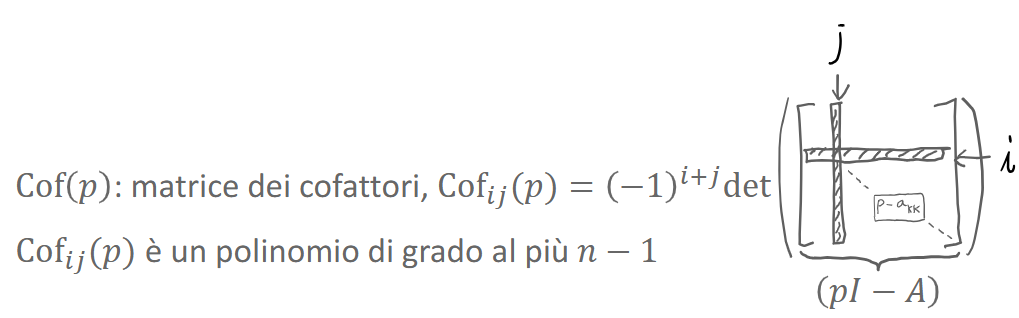
\includegraphics[width=0.7\linewidth]{immagini/2026-03-08-18-27-18.png}
    \end{figure}

Sostituendo $x$ nell'equazione di uscita, otteniamo:
$$ y = c^T \frac{\text{Cof}^T(p)}{\Delta_A(p)} b u + d u = \frac{c^T \text{Cof}^T(p) b + d \Delta_A(p)}{\Delta_A(p)} u $$
Moltiplicando tutto per $\Delta_A(p)$ si ottiene la relazione ingresso-uscita in forma polinomiale:
$$ \Delta_A(p)y = \underbrace{(c^T \text{Cof}^T(p) b + d \Delta_A(p))}_{N_A(p)} u $$
\textit{(Nota: $\Delta_A$ non dipende dalla coppia ingresso-uscita considerata, ma solo dalla matrice dinamica $A$).}

\subsubsection{Dunque $D = \Delta_A$ e $N = N_A$ è corretto?}
\begin{itemize}
    \item \textbf{SÌ}, se l'ordine dei modelli interno ed esterno coincidono.
    \item \textbf{NO}, se il modello esterno ha ordine inferiore di quello interno. Significa che si riesce a eliminare la $x$ dalla trasformazione d'uscita con un polinomio $D$ di grado inferiore a $\Delta_A$, ovvero sfruttando soluzioni $x_i = (\dots)u$ con a denominatore polinomi con solo \textit{parte} delle radici di $\Delta_A$.
\end{itemize}
$\implies$ Il modello corretto è quello che fa uso del polinomio $D$ di \textbf{grado minimo}.

\subsubsection{Esempi per il calcolo di $\Delta_A(p)$}
\textbf{Newton:}
$$ A = \begin{bmatrix} 0 & 1 \\ 0 & -\frac{h}{m} \end{bmatrix} \implies \Delta_A(p) = p^2 - \text{tr}(A)p + \det(A) = p^2 + \frac{h}{m}p $$

\textbf{Fibonacci:}
$$ A = \begin{bmatrix} 0 & 1 \\ 1 & 1 \end{bmatrix} \implies \Delta_A(p) = p^2 - p - 1 $$

\subsubsection{Esempio 1 (Sistemi non osservabili)}

\begin{figure}[H]
    \centering
    \begin{minipage}{0.3\textwidth}
        \centering
        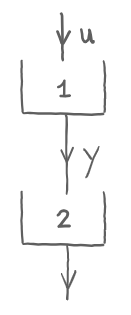
\includegraphics[width=0.5\linewidth]{immagini/2026-03-08-19-02-05.png}
    \end{minipage}\hfill
    \begin{minipage}{0.65\textwidth}
        $$ \begin{cases}
        \dot{x}_1 = u - k_1 x_1 \\
        \dot{x}_2 = k_1 x_1 - k_2 x_2
        \end{cases} \implies
        A = \begin{bmatrix} -k_1 & 0 \\ k_1 & -k_2 \end{bmatrix}, \quad b = \begin{bmatrix} 1 \\ 0 \end{bmatrix} $$
        $$ y = k_1 x_1 \implies c^T = \begin{bmatrix} k_1 & 0 \end{bmatrix}, \quad d = [0] $$
    \end{minipage}
\end{figure}

\textbf{Nota 1:} la variabile d'uscita $y$ è la portata uscente dal serbatoio 1. Dal punto di vista fisico, la portata uscente dal serbatoio 2 è l'uscita del sistema, nel senso di acqua che abbandona il sistema, ma non viene misurata. \\
\textbf{Nota 2:} la variabile di stato $x_2$ non influenza l'uscita $y$, quindi ci aspettiamo un modello esterno del primo ordine.

\textbf{Invertendo $(sI - A)$:}
$$ (sI - A) = \begin{bmatrix} s+k_1 & 0 \\ -k_1 & s+k_2 \end{bmatrix} \implies \text{Cof}^T = \begin{bmatrix} s+k_2 & 0 \\ k_1 & s+k_1 \end{bmatrix} $$
$$ \Delta_A(s) = (s+k_1)(s+k_2) $$
$$ N_A(s) = c^T \text{Cof}^T b + d \Delta_A = k_1(s+k_2) $$

\textbf{Conti "per sostituzione":}
$$ s x_1 = u - k_1 x_1 \implies (s+k_1)x_1 = u $$
$$ s x_2 = k_1 x_1 - k_2 x_2 $$
Sostituendo in $y = k_1 x_1$, moltiplichiamo tutto per $(s+k_1)$:
$$ (s+k_1)y = k_1(s+k_1)x_1 = k_1 u $$
Otteniamo il modello esterno effettivo:
$$ \underbrace{(s+k_1)}_{D} y = \underbrace{k_1}_{N} u $$

\noindent
\textbf{Nota 3:} $D$ è una \textit{parte} di $\Delta_A$ (le sue radici sono un sottoinsieme di quelle di $\Delta_A$; $D$ divide $\Delta_A$). \\
\textbf{Nota 4:} La radice di $\Delta_A$ che non è in $D$ è radice anche di $N_A$. È generale questo fatto? \textbf{SÌ}. \\
\textbf{Idea:} se, a conti fatti, trovo radici comuni tra $N_A$ e $\Delta_A$, posso eliminarle per ottenere i polinomi corretti $N$ e $D$? \textbf{NO}, vedi prossimo esempio.

\subsubsection{Esempio 2 (Sistemi non raggiungibili)}

\begin{figure}[H]
    \centering
    \begin{minipage}{0.3\textwidth}
        \centering
        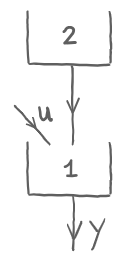
\includegraphics[width=0.5\linewidth]{immagini/2026-03-08-19-11-51.png}
    \end{minipage}\hfill
    \begin{minipage}{0.65\textwidth}
        $$ \begin{cases}
        \dot{x}_1 = u + k_2 x_2 - k_1 x_1 \\
        \dot{x}_2 = -k_2 x_2
        \end{cases} \implies
        A = \begin{bmatrix} -k_1 & k_2 \\ 0 & -k_2 \end{bmatrix}, \quad b = \begin{bmatrix} 1 \\ 0 \end{bmatrix} $$
        $$ y = k_1 x_1 \implies c^T = \begin{bmatrix} k_1 & 0 \end{bmatrix}, \quad d = [0] $$
    \end{minipage}
\end{figure}

\textbf{Nota 1:} la numerazione dei serbatoi è scelta in analogia all'esempio 1, per avere ingresso e uscita nel/dal serbatoio 1. \\
\textbf{Nota 2:} la variabile di stato $x_2$ influenza l'uscita $y$, ma non è influenzata dall'ingresso $u$. Vediamo questo cosa comporta...

\textbf{Invertendo $(sI - A)$:}
$$ (sI - A) = \begin{bmatrix} s+k_1 & -k_2 \\ 0 & s+k_2 \end{bmatrix} \implies \text{Cof}^T = \begin{bmatrix} s+k_2 & k_2 \\ 0 & s+k_1 \end{bmatrix} $$
Esattamente come nell'Esempio 1, otteniamo:
$$ \Delta_A(s) = (s+k_1)(s+k_2) $$
$$ N_A(s) = k_1(s+k_2) $$

\textbf{Conti "per sostituzione":}
$$ s x_1 = u + k_2 x_2 - k_1 x_1 \implies (s+k_1)x_1 = u + k_2 x_2 $$
$$ s x_2 = -k_2 x_2 \implies (s+k_2)x_2 = 0 \implies \text{ma attenzione: } x_2(t) = x_2(0)e^{-k_2 t} $$
Sostituendo in $y = k_1 x_1$, moltiplichiamo prima per $(s+k_1)$:
$$ (s+k_1)y = k_1(s+k_1)x_1 = k_1 u + k_1 k_2 x_2 $$
Moltiplicando ora per $(s+k_2)$:
$$ \underbrace{(s+k_1)(s+k_2)}_{D} y = \underbrace{k_1(s+k_2)}_{N} u + \underbrace{k_1 k_2 (s+k_2) x_2}_{= 0} $$
In questo caso, \textbf{non possiamo semplificare} $(s+k_2)$ a destra e a sinistra, altrimenti perderemmo l'informazione legata alle condizioni iniziali di $x_2$.

\subsection{Conclusioni Generali}

\begin{enumerate}
    \item L'ordine del modello ARMA (grado di $D$) è $\le$ di quello del modello interno (dimensione matrice $A$). Diciamo che $D$ è "contenuto" in (divide) $\Delta_A$, ovvero le sue radici sono autovalori di $A$.
    $$ D \subseteq \Delta_A \implies \Delta_A = D \cdot R $$
    $$ N \subseteq N_A = c^T \text{Cof}^T b + d \Delta_A \implies N_A = N \cdot R $$
    $R$ è il polinomio (monico) delle radici "sbagliate". 
    Vale il "contenuto stretto" (vedi es. 1) quando nel sistema ci sono delle variabili di stato (o loro combinazioni) che non hanno influenza sull'uscita. Il loro numero coincide con il grado di $R$.
    Si dice che ci sono variabili (o parti) del sistema \textbf{non osservabili}.

    \item Ci possono essere radici in comune tra $N$ e $D$:
    $$ N = n \cdot r, \quad D = d \cdot r $$
    $r$ è il polinomio (monico) delle radici comuni.
    Ciò accade (vedi es. 2) quando nel sistema ci sono delle variabili di stato (o loro combinazioni) che influenzano l'uscita ma non sono influenzate dall'ingresso. Il loro numero coincide con il grado di $r$.
    Si dice che ci sono variabili (o parti) del sistema \textbf{osservabili ma non raggiungibili}.

    \item Le radici "sbagliate" aggiungono delle soluzioni al modello che non esistono nel sistema fisico. Infatti, il modello ARMA "sbagliato" dell'es. 1 ha le soluzioni dell'es. 2. Se $x_2(0) \ne 0$, la soluzione non esiste nel sistema fisico dell'es. 1.
\end{enumerate}

\subsection{Zeri, Poli e Grado Relativo della Funzione di Trasferimento}

\textbf{FUNZIONE DI TRASFERIMENTO} (F.d.T., ce n'è una per ogni coppia $(y_i, u_j)$):
$$ G(p) = \frac{N(p)}{D(p)} = \frac{n(p)}{d(p)} \left( = \frac{c^T \text{Cof}^T(p) b + d \Delta_A(p)}{\Delta_A(p)} = c^T(pI - A)^{-1}b + d \right) $$

\textbf{NOTA:} il modello ARMA $dy = nu$ è detto (per analogia) di \textit{trasferimento}. Coincide col modello ARMA se $N$ e $D$ sono \textbf{coprimi} (senza radici in comune).

\begin{itemize}
    \item \textbf{Zeri e Poli:} radici di $n(p)$ e $d(p)$. In particolare, i poli sono autovalori di $A$ (non necessariamente tutti!).
    \item \textbf{Grado Relativo:} $r = \text{\#poli} - \text{\#zeri}$
\end{itemize}

Indicando con $n$ il numero di poli (sebbene possa essere $\le$ dell'ordine del modello interno e ARMA), possiamo scrivere la F.d.T. in forma fattorizzata:
$$ G(p) = \frac{\beta_r p^{n-r} + \beta_{r+1} p^{n-r-1} + \dots + \beta_{n-1} p + \beta_n}{p^n + \alpha_1 p^{n-1} + \dots + \alpha_{n-1} p + \alpha_n} = \beta_r \frac{(p - z_1)(p - z_2)\dots(p - z_{n-r})}{(p - p_1)(p - p_2)\dots(p - p_n)} $$

\textbf{NOTA:} zeri (rappresentati con pallini $\circ$) e poli (rappresentati con crocette $\times$) possono essere a coppie complessi coniugati.

\begin{figure}[htbp]
    \centering
    % \includegraphics[width=0.6\textwidth]{piano_complesso_poli_zeri.png}
    \vspace{4cm} % Spazio vuoto temporaneo
    \caption{INSERIRE QUI L'IMMAGINE: [Piano complesso Re-Im con rappresentazione di poli e zeri, coordinate $a, \omega$ e coordinate polari $\omega_n, \theta$]}
\end{figure}

Nel piano complesso:
$$ p_k = a + i\omega = \omega_n e^{i\theta} = \omega_n (\cos(\theta) + i \sin(\theta)) $$
A tempo continuo (t.c.): lo \textbf{smorzamento} è $\xi = \cos(\pi - \theta)$, la \textbf{pulsazione naturale} è $\omega_n = |p_k|$.
$$ (s - p_k)(s - \bar{p}_k) = s^2 - 2as + |p_k|^2 = s^2 + 2\xi\omega_n s + \omega_n^2 $$

\subsubsection{Esempi di calcolo di zeri e poli}
\textbf{NEWTON:} 
$$ G(s) = \frac{1}{ms(s+h/m)} $$
Zeri: nessuno. Poli: $p_1 = 0$ e $p_2 = -\frac{h}{m}$.

\textbf{FIBONACCI:}
$$ D(z) = -\frac{z+1}{z^2-z-1} $$
Zeri: $z_1 = -1$. Poli: $p_{1,2} = \frac{1 \pm \sqrt{5}}{2}$ (dove la radice positiva corrisponde alla sezione aurea).

\subsection{Passaggio da Modello Esterno a Interno (Realizzazione del modello ARMA)}

\subsubsection{Un Caso Particolare}
Se $\beta_0 = \beta_1 = \dots = \beta_{n-1} = 0$ (ovvero, non ci sono derivate o anticipi dell'ingresso):
$$ \text{ARMA: } p^n y + \alpha_1 p^{n-1} y + \dots + \alpha_n y = \beta_n u $$

In questo caso, una realizzazione "naturale" (matrice compagna) dello stato è:
\begin{align*}
x_1 &= y \\
px_1 &= py = x_2 \\
px_2 &= p^2y = x_3 \\
\vdots \\
px_{n-1} &= p^{n-1}y = x_n \\
px_n &= p^ny = -\alpha_n x_1 - \dots - \alpha_1 x_n + \beta_n u
\end{align*}

In forma matriciale:
$$ A = \begin{bmatrix} 
0 & 1 & 0 & \dots & 0 \\ 
0 & 0 & 1 & \dots & 0 \\ 
\vdots & \vdots & \vdots & \ddots & \vdots \\ 
0 & 0 & 0 & \dots & 1 \\ 
-\alpha_n & -\alpha_{n-1} & \dots & \dots & -\alpha_1 \end{bmatrix}, \quad 
b = \begin{bmatrix} 0 \\ \vdots \\ 0 \\ \beta_n \end{bmatrix} $$
$$ c^T = \begin{bmatrix} 1 & 0 & \dots & 0 \end{bmatrix}, \quad d = [0] $$

\textbf{Esempio (Newton):} $x_1 = y$ (posizione), $x_2 = \dot{y}$ (velocità).
$$ A = \begin{bmatrix} 0 & 1 \\ -\alpha_2 & -\alpha_1 \end{bmatrix} = \begin{bmatrix} 0 & 1 \\ 0 & -\frac{h}{m} \end{bmatrix}, \quad b = \begin{bmatrix} 0 \\ \beta_2 \end{bmatrix} = \begin{bmatrix} 0 \\ \frac{1}{m} \end{bmatrix} $$
$$ c^T = \begin{bmatrix} 1 & 0 \end{bmatrix}, \quad d = [0] $$

\subsubsection{La Forma Canonica di Ricostruzione (Caso Generale)}
È una "ricetta" generale per ricavare un modello interno a partire dal modello ARMA:
$$ (p^n + \alpha_1 p^{n-1} + \dots + \alpha_n)y(t) = (\beta_0 p^n + \beta_1 p^{n-1} + \dots + \beta_n)u(t) $$

Le matrici della forma canonica (indicata con il pedice $r$) sono:
$$ A_r = \begin{bmatrix} 
0 & 0 & \dots & 0 & -\alpha_n \\ 
1 & 0 & \dots & 0 & -\alpha_{n-1} \\ 
0 & 1 & \dots & 0 & -\alpha_{n-2} \\ 
\vdots & \vdots & \ddots & \vdots & \vdots \\ 
0 & 0 & \dots & 1 & -\alpha_1 \end{bmatrix}, \quad 
b_r = \begin{bmatrix} \gamma_n \\ \gamma_{n-1} \\ \gamma_{n-2} \\ \vdots \\ \gamma_1 \end{bmatrix} $$
$$ c_r^T = \begin{bmatrix} 0 & 0 & \dots & 0 & 1 \end{bmatrix}, \quad d_r = [\beta_0] $$

Dove i parametri $\gamma_i$ sono calcolati come:
$$ \gamma_i = \beta_i - \beta_0 \alpha_i $$

\paragraph{Che variabili di stato utilizza?}
Dalla trasformazione d'uscita si ha $y = z_n + \beta_0 u \implies z_n = y - \beta_0 u$.
Le equazioni di definizione delle variabili di stato $z_i$ sono ricorsive:
\begin{align*}
z_{n-1} &= (p + \alpha_1)y - (\beta_0 p + \beta_1)u \\
&\vdots \\
z_i &= (p^{n-i} + \alpha_1 p^{n-i-1} + \dots + \alpha_{n-i})y - (\beta_0 p^{n-i} + \beta_1 p^{n-i-1} + \dots + \beta_{n-i})u \\
&\vdots \\
z_1 &= (p^{n-1} + \alpha_1 p^{n-2} + \dots + \alpha_{n-1})y - (\beta_0 p^{n-1} + \beta_1 p^{n-2} + \dots + \beta_{n-1})u
\end{align*}

\textbf{NOTA 1:} le variabili di stato sono combinazioni di $y(t)$ e $u(t)$ e loro derivate a t.c. o anticipi a t.d., $p^k y(t)$ (ad es., nella formulazione interna di Newton: posizione $x_1 = y$ e velocità $x_2 = dy/dt$). \\
\textbf{NOTA 2:} Può sembrare che contengano valori futuri di $y$ e $u$ (t.d. $p y(t) = y(t+1)$), ma non è così. Grazie al legame del mod. ARMA sono combinazioni che dipendono dal passato di $y$ e $u$.

\paragraph{Dimostrazione della dipendenza dal passato}
Dividendo l'equazione ARMA per potenze di $p$, si dimostra che ogni $z_i$ dipende solo da valori passati (potenze negative di $p$):
\begin{align*}
\text{ARMA}/p^n \implies & z_n = y - \beta_0 u = -(\alpha_1 p^{-1} + \dots + \alpha_n p^{-n})y(t) + (\beta_1 p^{-1} + \dots + \beta_n p^{-n})u(t) \\
\text{ARMA}/p^{n-1} \implies & z_{n-1} = (p + \alpha_1)y - (\beta_0 p + \beta_1)u = -(\alpha_2 p^{-1} + \dots)y + (\beta_2 p^{-1} + \dots)u \\
\vdots \\
\text{ARMA}/p \implies & z_1 = \dots = -\alpha_n p^{-1} y + \beta_n p^{-1} u
\end{align*}

\paragraph{Verifica delle equazioni di stato}
Calcolando l'operatore $p$ sulla definizione di $z_i$:
$$ pz_i = (p^{n-i+1} + \alpha_1 p^{n-i} + \dots + \alpha_{n-i} p + \alpha_{n-i+1} - \alpha_{n-i+1})y - (\beta_0 p^{n-i+1} + \dots + \beta_{n-i} p + \beta_{n-i+1} - \beta_{n-i+1})u $$
Isolando i termini si ottiene l'aggiornamento di stato voluto:
\begin{itemize}
    \item Per $i > 1$: $pz_i = z_{i-1} - \alpha_{n-i+1}(z_n + \beta_0 u) + \beta_{n-i+1} u = z_{i-1} - \alpha_{n-i+1} z_n + \underbrace{(\beta_{n-i+1} - \beta_0 \alpha_{n-i+1})}_{\gamma_{n-i+1}}u$
    \item Per $i = 1$: $pz_1 = (0) - \alpha_n(z_n + \beta_0 u) + \beta_n u = -\alpha_n z_n + \underbrace{(\beta_n - \beta_0 \alpha_n)}_{\gamma_n}u$
\end{itemize}
\textit{Questo dimostra esattamente la struttura della matrice $A_r$ e del vettore $b_r$.}

\subsubsection{Esempi di Realizzazione e Cambio di Variabili}

\paragraph{Esempio: Newton}
Con $\alpha_1 = \frac{h}{m}$, $\alpha_2 = 0$, $\beta_0 = 0$, $\beta_1 = 0$, $\beta_2 = \frac{1}{m}$:
$$ A_r = \begin{bmatrix} 0 & -\alpha_2 \\ 1 & -\alpha_1 \end{bmatrix} = \begin{bmatrix} 0 & 0 \\ 1 & -\frac{h}{m} \end{bmatrix}, \quad
b_r = \begin{bmatrix} \beta_2 \\ \beta_1 \end{bmatrix} = \begin{bmatrix} \frac{1}{m} \\ 0 \end{bmatrix} $$
$$ c_r^T = \begin{bmatrix} 0 & 1 \end{bmatrix}, \quad d_r = \beta_0 = 0 $$

Nota: le variabili $z_i$ di solito non sono le variabili di stato $x_i$ scelte nella formulazione interna, ma sono una buona scelta di stato. Ciò significa che c'è un legame lineare invertibile tra le $z$ e le $x$:
$$ \begin{cases} 
z_1 = \dot{y} + \alpha_1 y - \beta_0 \dot{u} - \beta_1 u = \dot{y} + \frac{h}{m}y = x_2 + \frac{h}{m}x_1 \\ 
z_2 = y - \beta_0 u = y = x_1 
\end{cases} $$

In forma matriciale: $z = Tx \implies x = T^{-1}z$
$$ T = \begin{bmatrix} \frac{h}{m} & 1 \\ 1 & 0 \end{bmatrix}, \quad T^{-1} = \frac{1}{-1} \begin{bmatrix} 0 & -1 \\ -1 & \frac{h}{m} \end{bmatrix} = \begin{bmatrix} 0 & 1 \\ 1 & -\frac{h}{m} \end{bmatrix} $$

La trasformazione $z = Tx$ ($T$: matrice $n \times n$ non singolare) è un \textbf{cambio di variabili di stato}. Corrisponde ad un cambio di coordinate (di base) nello spazio di stato. \\
\textit{Nota:} ci sono quindi infinite scelte di variabili di stato, una per ogni possibile matrice di trasformazione $T$, a partire da una data scelta $x$. A partire da tutte le corrispondenti realizzazioni $(A, b, c^T, d)$ si ottiene lo stesso modello esterno $Dy = Nu$.

\paragraph{Esempio: Fibonacci}
Con $\alpha_1 = -1$, $\alpha_2 = -1$, $\beta_0 = 0$, $\beta_1 = -1$, $\beta_2 = -1$:
$$ A_r = \begin{bmatrix} 0 & 1 \\ 1 & 1 \end{bmatrix}, \quad b_r = \begin{bmatrix} -1 \\ -1 \end{bmatrix}, \quad c_r^T = \begin{bmatrix} 0 & 1 \end{bmatrix}, \quad d_r = 0 $$

Legame tra le $z$ e le $x$ ($x_1 =$ coppie giovani; $x_2 =$ coppie adulte):
$$ z_1(t) = y(t+1) + \alpha_1 y(t) - \beta_0 u(t+1) - \beta_1 u(t) = y(t+1) - y(t) + u(t) $$
Sostituendo il modello interno:
$$ z_1(t) = x_1(t+1) + x_2(t+1) - (x_1(t) + x_2(t)) + u(t) = x_2(t) + x_1(t) + x_2(t) - u(t) - x_1(t) - x_2(t) + u(t) = x_2(t) $$
$$ z_2(t) = y(t) - \beta_0 u(t) = y(t) = x_1(t) + x_2(t) $$

In forma matriciale:
$$ z = Tx \implies T = \begin{bmatrix} 0 & 1 \\ 1 & 1 \end{bmatrix}, \quad T^{-1} = \frac{1}{-1} \begin{bmatrix} 1 & -1 \\ -1 & 0 \end{bmatrix} = \begin{bmatrix} -1 & 1 \\ 1 & 0 \end{bmatrix} $$
\textit{Nota:} ricordiamoci anche la formulazione con $x_1 = \text{totale coppie}$ e $x_2 = \text{coppie adulte}$. Ricavare la $T$ in quel caso è un ottimo esercizio.

\subsection{Il Cambio di Variabili (di Stato): Interpretazione Geometrica}
$$ z = Tx, \quad x = T^{-1}z $$

\begin{itemize}
    \item \textbf{Colonne di $T^{-1}$:}
    Se consideriamo il versore $z = e^{(i)} = \begin{bmatrix} 0 & \dots & 1 & \dots & 0 \end{bmatrix}^T$ (con l'$1$ in posizione $i$), allora $x = T^{-1}e^{(i)} = i\text{-esima colonna di } T^{-1}$.
    La colonna rappresenta il versore dell'asse $z_i$ espresso nelle coordinate $x$.

    \item \textbf{Righe di $T$:} Combinazione di $x$ che definisce $z_i$.
    $$ z_i = [\text{riga } i\text{-esima di } T] \cdot x $$
    $$ \frac{\partial z_i}{\partial x} = \nabla z_i = \text{riga } i\text{-esima di } T $$
    Il vettore gradiente $\nabla z_i$ è perpendicolare ($\perp$) alle linee di livello costanti di $z_i$ ed è perpendicolare ($\perp$) agli assi $z_j$ per $j \neq i$.
\end{itemize}

\begin{figure}[htbp]
    \centering
    % \includegraphics[width=0.7\textwidth]{interpretazione_geometrica_cambio_variabili.png}
    \vspace{5cm} % Spazio vuoto temporaneo
    \caption{INSERIRE QUI L'IMMAGINE: [Piano cartesiano $x_1, x_2$ con i nuovi assi $z_1, z_2$ e i vettori gradiente per il sistema di Newton]}
\end{figure}

\subsection{Come Cambiano le Equazioni del Sistema}
Applichiamo il cambio di coordinate all'equazione di stato $px = Ax + bu$:
$$ pz = T(px) = T(Ax + bu) = TAT^{-1}z + Tbu = \underbrace{\tilde{A}}_{TAT^{-1}}z + \underbrace{\tilde{b}}_{Tb}u $$
E all'equazione della trasformazione d'uscita:
$$ y = c^Tx + du = c^TT^{-1}z + du = \underbrace{\tilde{c}^T}_{c^TT^{-1}}z + du $$

\textbf{Nota:} calcolando il modello ARMA o la F.d.T. a partire da queste equazioni (con le matrici "tilde"), si ottiene lo stesso risultato ottenuto con le variabili $x$ originali (con le matrici $A, b, c^T, d$).
$$ G(p) = c^T(pI - A)^{-1}b + d $$
$$ \tilde{G}(p) = \tilde{c}^T(pI - \tilde{A})^{-1}\tilde{b} + d = c^TT^{-1}(pI - TAT^{-1})^{-1}Tb + d $$
Sfruttando la proprietà $(T(pI - A)T^{-1})^{-1} = T(pI - A)^{-1}T^{-1}$, si semplifica in:
$$ \tilde{G}(p) = c^T T^{-1} T (pI - A)^{-1} T^{-1} T b + d = c^T(pI - A)^{-1}b + d = G(p) $$

In particolare, i polinomi caratteristici di $A$ e $TAT^{-1}$ coincidono (poiché sono matrici simili):
$$ \Delta_{\tilde{A}}(p) = \det(pI - TAT^{-1}) = \det(T(pI - A)T^{-1}) = \det(T)\det(pI - A)\det(T^{-1}) = \Delta_A(p) $$

\section{Riassumendo...}

\begin{itemize}
    \item \textbf{Modello Interno} (per sistema SISO):
    \begin{itemize}
        \item t.c.: $\dot{x} = Ax + bu$
        \item t.d.: $x(t+1) = Ax(t) + bu(t)$
    \end{itemize}
    $$ y(t) = c^T x(t) + d u(t) $$

    \item \textbf{Modello Esterno} (ARMA):
    $$ \underbrace{(p^n + \alpha_1 p^{n-1} + \dots + \alpha_n)}_{D(p)} y(t) = \underbrace{(\beta_0 p^n + \beta_1 p^{n-1} + \dots + \beta_n)}_{N(p)} u(t) $$

    \item \textbf{Funzione di Trasferimento} (F.d.T.):
    $$ G(p) = \frac{N(p)}{D(p)} = \frac{n(p)}{d(p)} \left( = \frac{c^T \text{Cof}^T(p) b + d \Delta_A(p)}{\Delta_A(p)} = c^T(pI - A)^{-1}b + d \right) $$
\end{itemize}

\begin{figure}[htbp]
    \centering
    % \includegraphics[width=0.8\textwidth]{riassunto_tre_formulazioni.png}
    \vspace{4cm} % Spazio vuoto temporaneo
    \caption{INSERIRE QUI L'IMMAGINE: [Schema finale riassuntivo "TRE FORMULAZIONI E LORO RELAZIONI" con i passaggi "facile", "banale" e "ricetta facile"]}
\end{figure}






\end{document}